\documentclass[thesis.tex]{subfile}
\begin{document}
\chapter{Distributed State Estimation} \label{ch:Distributed State Estimation}
This chapter describes the distributed state estimation system created with the robot\_localization package~\cite{MooreStouch2014, Moore}. The overarching concept behind this system is for individual robots to use their sensor data to create pose estimates for the other robots in their environment. The pose estimates are then sent to the other robots and integrated into their own personal pose estimate, allowing for more accurate localization.
  
\section{Theory} \label{Theory}
With more sensor inputs to a \gls{kf}, noise can usually be removed more accurately. One way to increase the number of sensor inputs to a filter is to add more sensors to the robot. However, this will rapidly drive up cost and complexity. Another solution is to have robots share their information about the surrounding world, thus artificially inflating the number of sensors a robot has.

The flow for this distributed system for sharing sensor information is as follows. A robot at position $p_l$, where $l$ represent that this position is with respect to the local frame, detects another robot at position $g_l$. The robot at $p_l$ then calculates its pose in with respect to the global frame, $p_g$ and then transforms $g_l \rightarrow g_g$. This position $g_g$ is then shared with the robots in the surrounding environment, which integrate the position into their own localization estimate. This is summarized in \cref{tab:external_pose}.

\begin{table}[htbp]
\centering
\begin{align}
&\text{\gls{kf} output} \rightarrow p_l, p_g \\
&\text{Lidar scan} + p_l \rightarrow g_l \\
&g_g \rightarrow \text{\gls{kf} input}
\end{align}
\caption{General algorithm for computing external pose.}
\label{tab:external_pose}
\end{table}

\subsection{Assumptions and Constraints}
In developing this distributed state estimation system, we have made these assumptions and imposed these constraints on the environment and robots.

\begin{itemize}
\item An arbitrary number independent mobile robots operating in a planar environment
\item Wireless communication abilities between some robots in the environment
\item No known static map of environment
\item \gls{gps} and a compass for localization in the world frame is available
\item Motion planning and control of other robots is unknown and unpredictable
\item Robots run on the \gls{ros} platform and use standard \gls{ros} practices and constructs
\end{itemize}

These assumptions and constraints approximate a robot operating in an unknown environment with unknown other agents. We do not make an assumption of cooperation with other robots with respect to path planning or control in order to increase state estimate accuracy. Further, we assume there is no static map, preventing the use of static landmarks to increase accuracy.

\section{Methods}
The following sections describes how the position estimates $p_l$, $p_g$, $g_l$, and $g_g$ are obtained.

\subsection{Coordinate Systems}
First, it is necessary to understand the naming terminology for the coordinate systems used in this discussion. The system used is identical to the \gls{ros} standard, REP-105~\cite{REP_105}. There are three different coordinate frames: $map$, $odom$, and $base\_link$.

\subsubsection{Base\_Link Frame}
The base\_link frame is the simplest to understand. It is a rigidly fixed frame attached to the base of the mobile robot, often at the center. This frame can be used to describe the position of different parts of the robot in reference to itself. For example, no matter where the robot moves, the Kinect camera will always be in the same position relative to the base\_link frame. On the TurtleBot, the base\_link frame defined by REP-105 is called base\_footprint, and there is a separate base\_link frame. The names base\_footprint and base\_link are used interchangeably in this thesis. 

\subsubsection{Odom Frame}
The odom frame is a fixed world frame. Its origin is at the starting point of the robot, and thus the $odom \rightarrow base\_link$ transformation represents the position of the robot relative to its starting point. This frame is subject to drift over time due to error accumulation. These errors could be systematic or random, and have no bounds. However, this frame is guaranteed to be continuous. Generally, the $odom \rightarrow base\_link$ is calculated using wheel encoders and/or an IMU. Because it is continuous, it is a good reference frame for short term navigation. However, due to drift it is not useful for long-term localization. Other names for the odom frame are local frame and odometry frame.

\subsubsection{Map Frame}
The map frame is also a fixed world frame. What distinguishes it from the odom frame is that it is not continuous but it is also not subject to drift over time. The presence of discrete changes make it a poor choice for navigation and short term planning, but the lack of drift makes it valuable for long-term localization. Other names for the map frame are world frame and global frame.
 
\subsection{Filters}
There are two filters operating on the robot to create a whole localization estimate. The first is the \gls{con_filter}, and the second is the \gls{disc_filter}. They each perform a separate but related localization task, and combined give a full localization estimate with respect to both the local and global frames of the robot. 

\subsubsection{Continuous Filter} \label{con_filter_subsubsection}
The \gls{con_filter} calculates and publishes the transformation from $odom \rightarrow base\_link$. It receives odometry information from the robot's wheel encoders. %and IMU
.
%Another name for the \gls{con_filter} is the \gls{self_filter}.  

\subsubsection{Discrete Filter} \label{disc_filter_subsubsection}
The \gls{disc_filter} calculates the transformation from $map \rightarrow base\_link$. Because the \gls{ros} TF package that handles coordinate frame transformations enforces a tree structure where each node can only have one parent, the \gls{disc_filter} references the $odom \rightarrow base\_link$ transform published by the \gls{con_filter} and publishes a transform from $map \rightarrow odom$. The inputs to the \gls{disc_filter} are the robot's wheel encoder odometry, %IMU readings,
a \gls{gps}, and external poses calculated by other robots ($g_g$ as described in \cref{Theory}).
%Another name for the \gls{disc_filter} is the \gls{dist_filter}.

\subsubsection{\gls{ekf} vs \gls{ukf}}
The robot\_localization package allows for seamless switching between a \gls{ekf} and \gls{ukf}. For these simulations a \gls{ukf} was used for all filters due to its simpler nature, lower computational requirements, and higher accuracy in non-linear systems, however no methods presented here would conflict with the choice of an \gls{ekf} instead.
 
\subsubsection{Inputs and Outputs}
The general inputs of each filter have been listed previously in each filter description. The robot\_localization package allows the user to choose which information to fuse into the localization estimate from each sensor input. For any input, the following readings can be fused while operating in 2D:
\begin{itemize}
\item X and Y position
\item Yaw
\item X and Y velocity
\item Yaw velocity
\item X and Y acceleration
\end{itemize}
Choosing which of these inputs to use is robot specific and will change between simulation and real world testing. For our simulations, we fused x, y, and yaw velocity from odometry into both the \gls{con_filter} and \gls{disc_filter}. For the fused \gls{gps} and external pose inputs for the \gls{disc_filter} we fused the x and y position.
 
\subsection{ROS Node Structure}
\Cref{fig:node_graph} shows the basic structure of the \gls{ros} nodes running on the TurtleBot. All nodes have the ``/turtlebot1/" namespace appended to them to separate out multiple robots during simulation. In a 3 robot simulation there would be identical copies of this graph with the ``/turtlebot2/" and ``/turtlebot3/" namespace. As such, a node with name ``/turtlebot1/fake\_node" will be referred to as ``fake\_node" for the sake of brevity.
 
%TODO I should update this with the new graph
\begin{landscape}
\begin{figure}[p]
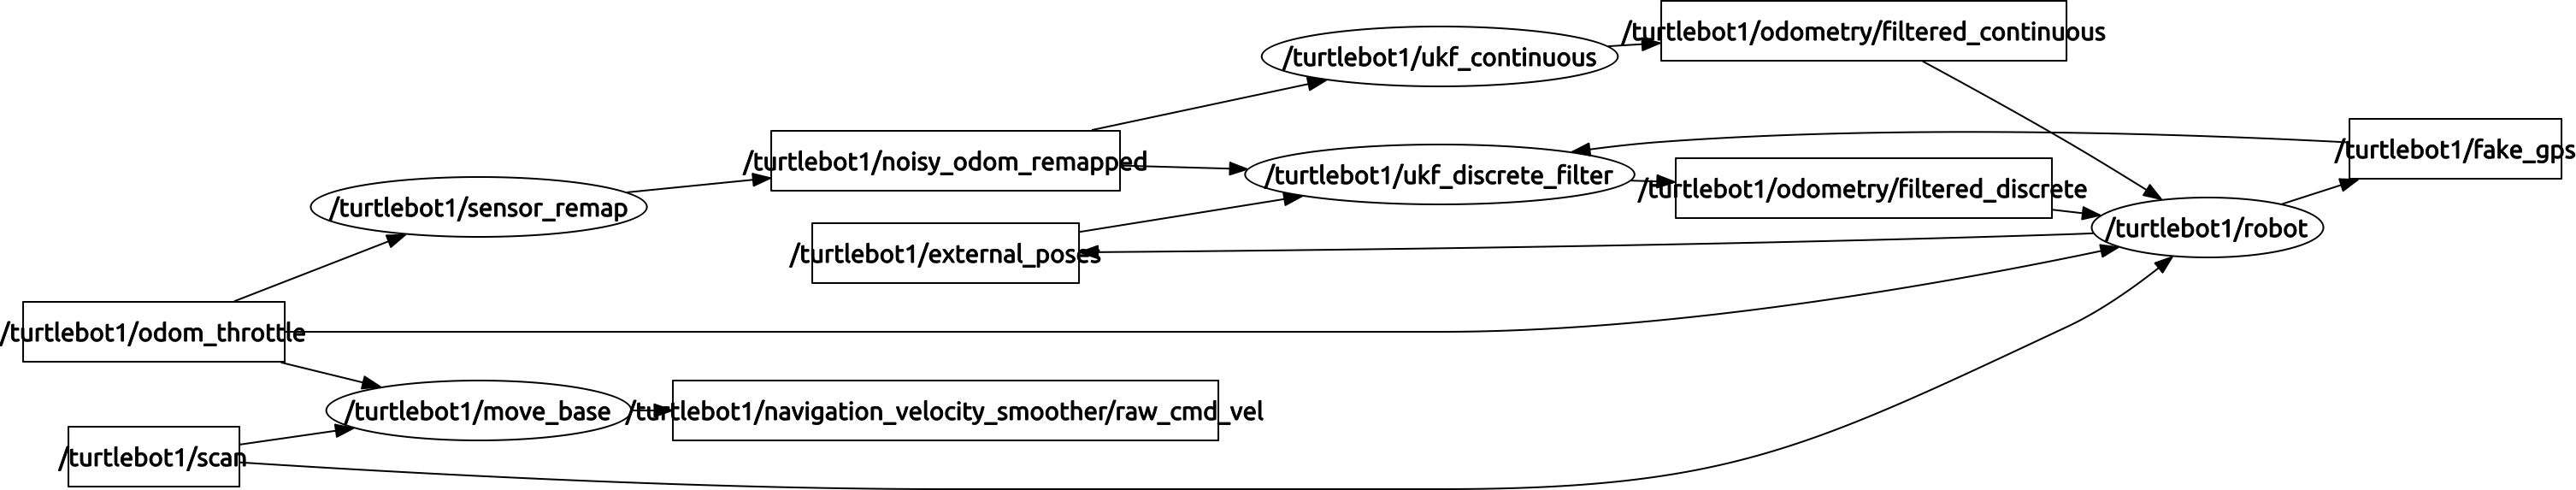
\includegraphics[width=\paperwidth, keepaspectratio]{simple_rosgraph}
\caption{ROS Node Structure. Nodes are enclosed in rectangles, topics are enclosed in ovals.}
\label{fig:node_graph}
\end{figure}
\end{landscape}

\subsubsection{Robot Node}
The robot node is where most of the heavy lifting is done. This node listens to the Lidar and odometry information, and calculates the external poses that are sent to other robots. It also sends movement commands to the move\_base node, but this is done via an action server and not a topic so it is not shown in \cref{fig:node_graph}. The robot node also publishes the simulated \gls{gps} (fake\_gps) based on the robot's odometry information that is sent to the \gls{disc_filter}.

\subsubsection{Sensor Remap Node}
The sensor\_remap node subscribes to the odom topic, which is produced by the Gazebo simulator, and adds noise. The noise model is described in \cref{sec:noise_model}. This node also remaps topic frame\_ids to handle some multi-robot simulation peculiarities as explained in \cref{sec:sim_details}.

\subsubsection{Filter Nodes}
The \gls{disc_filter} and \gls{con_filter} are both subscribed to the odometry information, and the \gls{disc_filter} is additionally subscribed to the external poses and \gls{gps}.

\subsubsection{Move\_Base Node}
The move\_base node is the \gls{ros} navigation stack node. It subscribes to the scan topic for the creation of the local costmap and to the odom topic for path planning purposes. It publishes a raw velocity command which is then sent to the velocity smoother as described in \cref{sec:controls}.

\subsubsection{Unvisualized Nodes}
There are some unvisualized nodes. They are listed here along with their function.
\begin{itemize}
\item Simulation Timer - Allows user to set a specific runtime for simulations and stops simulation once that time has been exceeded
\item cmd\_vel\_mux - Described in \cref{sec:controls}
\item depthimage\_to\_laserscan - Emulates a Lidar using the Microsoft Kinect point cloud data~\cite{Rockey2016}
\item gazebo\_odom\_throttle - By default Gazebo publishes odometry at 1000Hz, node throttles this down to more realistic 10Hz
\item kobuki\_safety\_controller - Described in \cref{sec:controls}
\item navigation\_velocity\_smoother - Described in \cref{sec:controls}
\item sensor\_record - Records sensor and filter outputs to \gls{CSV} files for later analysis.
\item static\_tf\_publisher - Publishes transforms to circumvent multi-robot simulation errors described in \cref{sec:sim_details}.
\end{itemize}

\subsection{Communications Logic}
In \gls{ros}, there are three separate methods for communication between nodes: publish/subscribe, services, and action servers. This section will describe these three methods, and explain which parts of the system use which method and the justification for this decision.

\subsubsection{Publish/Subscribe}
The publish/subscribe method for inter-node communication is the simplest of the three available. A node declares a topic name and message type, and then sends out messages on that topic. The \gls{roscore} registers what node is publishing the topic, and later facilitates any subscription attempts to the topic. There is no communication between the publisher and the subscriber. The publisher does not know how many subscribers are present, if any, or if they are receiving the messages. The subscriber does not have any way to send feedback back to the publisher about the messages received. This system is best used for data that is always being continuously published, such as sensor measurements, and there is no need for two-way communication. Publish/subscribe also has the least overhead of any method.

\subsubsection{Services}
Services are a middle ground between action servers and publish/subscribe. One way of describing services is ``Request/Reply"~\cite{RosServices}. A service message is described, and then a client is able to send a request in the style of that message to the service server. The server then responds with an answer. This service call blocks other actions from happening within the calling node while it waits for a response from the server, and the server cannot provide feedback while it is processing the response. This makes services suitable for fast operations that will not cause delays in other parts of the program.

\subsubsection{Action Servers}
Action servers are the most robust communication option. Similar to a service, there is a server and client relationship. In an action server, the call to the server is non-blocking, and the server can provide feedback during the operation. Additionally, the client can request that a call to an action server be canceled or replaced with a newer call. This makes action servers appropriate for communications that may take a long time or where extra feedback to the calling client could be valuable.

\subsubsection{Communication Choices}
All sensor measurements, and all robot\_localization filter inputs and outputs, are done via the publish/subscribe methodology. It does not matter if any \gls{node} is listening to the sensor, and there can be no two-way communication, so this should be obvious. Communication with the move\_base navigation stack is done via an action server. Both of these communications were not choices made for this thesis, they are previously defined functionality of the software packages.

For sharing external poses, multiple options were considered. The filter input must be a published topic, so at some point publish/subscribe must be used. However, there cannot be multiple publishers of the same topic, so the filters would need to have an input for each robot in the environment, or there would have to be a secondary communication layer on top. Inputs cannot be dynamically created and deleted in the robot\_localization package, they must be declared before runtime in a launch file. Therefore having an input for each robot would conflict with our goal of handling the addition and removal of robots dynamically from \cref{sec:Problem Statement}.

%TODO get rid of this in all of paper
Thus, an extra communications layer is needed. Receiving an external pose and publishing it back to a topic should be an extremely fast operation. So a service may seem like a reasonable choice, but we chose an action server instead for two reasons. First, even though the requested operation should be very fast, the service is still a blocking call. This may not be an issue when there are only a few robots in the environment, but as the number of robots increases, the delay between sending out external pose measurements and receiving them back also increases. This could lead to issues in very robot dense environments. Second, while no feedback is currently needed, the opportunity for feedback is advantageous in further developments of this system. Each robot runs an action server that can receive external poses, and also maintains a list of action clients for every other robot in the environment to send poses to those robot's servers. This action client list is dynamically expanded and pruned at a set time interval, satisfying our goals from \cref{sec:Problem Statement}.

\subsection{Gazebo Simulation Details} \label{sec:sim_details}
Gazebo and the TurtleBot simulation files are not designed to handle multi-robot simulations easily, so some modifications were required to make everything work.

One issue is that the tf package, which handles coordinate frame transformations in \gls{ros}, enforces a tree structure, as noted in \cref{disc_filter_subsubsection}. This means that each frame has one and only one parent. By default, Gazebo publishes the $odom \rightarrow base\_link$ transform for the TurtleBot model. This is necessary and cannot be disabled, because the Gazebo odometry represents the ground truth of the robot. However, this means that the \gls{con_filter} cannot publish the same transform or there will be an error of conflicting authority. To circumvent this, a static transform publisher creates a new frame called ``base\_footprint\_filter". This frame represents the location of the robot according to the filter. The \gls{con_filter} publishes the transform $odom \rightarrow base\_footprint\_filter$. This also means that we can establish that $p_{\text{base\_footprint}} - p_{\text{base\_footprint\_filter}} = \text{error}_{\text{continuous\_filter}}$.

Another issue is caused by conflicting node names. Each robot runs the exact same nodes, and only one \gls{ros} master is used for the simulations. This is avoided by using namespaces in the launch files, where every node name is prefixed by ``turtlebotX". The same is done with the \gls{urdf} of the TurtleBot model; prefixing every joint and link name with a robot specific identifier prevents naming collisions.

\subsection{Noise Model} \label{sec:noise_model}
Gazebo is a relatively noiseless simulation, which makes adding noise a requirement. The following sections describe the noise models implemented in the simulation.

\subsubsection{Odometry}
For the odometry, the noise model was taken from Probabilistic Robotics by \textcite[136]{ProbabilisticRobotics}. In Table 5.6 they show the algorithm for sampling from $p(x_t \mid u_t, x_{t-1})$, where $x_t$ represents the pose at time $t$ and $u_t$ represents the odometry measurement received. This table is reproduced in \cref{tab:sample_motion_model_odometry}.

\begin{table}[htbp]
\centering
\begin{align}
&\delta_{\text{rot1}} = \text{atan2}(\bar{y}' - \bar{y}, \bar{x}' - \bar{x}) - \bar{\theta}\\ 
&\delta_{\text{trans}} = \sqrt{(\bar{x} - \bar{x}')^2 + (\bar{y} - \bar{y}')^2}\\
&\delta_{\text{rot2}} = \bar{\theta}' - \bar{\theta} - \delta_{\text{rot1}}\\
\notag \\
&\hat{\delta}_{\text{rot1}} = \delta_{\text{rot1}} - \textbf{sample}(\alpha_1\lvert\delta_{\text{rot1}}\rvert + \alpha_2\delta_{\text{trans}})\\
&\hat{\delta}_{\text{trans}} = \delta_{\text{trans}} - \textbf{sample}(\alpha_3\delta_{\text{trans}} + \alpha_4(\lvert\delta_{\text{rot1}}\rvert + \lvert\delta_{\text{rot2}}\rvert)\\
&\hat{\delta}_{\text{rot2}} = \delta_{\text{rot2}} - \textbf{sample}(\alpha_1\lvert\delta_{\text{rot2}}\rvert + \alpha_2\delta_{\text{trans}})\\
\notag \\
&x' = x + \hat{\delta}_{\text{trans}}\cos(\theta + \hat{\delta}_{\text{rot1}})\\
&y' = y + \hat{\delta}_{\text{trans}}\sin(\theta + \hat{\delta}_{\text{rot1}})\\
&\theta' = \theta + \hat{\delta}_{\text{rot1}} + \hat{\delta}_{\text{rot2}}\\
\notag \\
&return \ x_t = (x', y', \theta')^T
\end{align}
\caption[Algorithm sample\_motion\_model\_odometry]{Algorithm for sampling from $p(x_t \mid u_t, x_{t-1})$ based on odometry information. Here the pose at time $t$ is represented by $x_{t-1} = (x\ y\ \theta)^T)$. The control is a differentiable set of two pose estimates obtained by the robot's odometer, $u_t = (\bar{x}_{t-1}\ \bar{x}_t)^T$, with $\bar{x}_{t-1} = (\bar{x}\ \bar{y}\ \bar{\theta})$ and $\bar{x}_{t} = (\bar{x}'\ \bar{y}'\ \bar{\theta}')$}
\label{tab:sample_motion_model_odometry}
\end{table} 

In this model, a movement by the robot (represented by two odometry readings, $\bar{x}_{t-1} = (\bar{x}\ \bar{y}\ \bar{\theta})$, $\bar{x}_{t} = (\bar{x}'\ \bar{y}'\ \bar{\theta}')$) is represented by a sequence of three motions: a rotation, translation, and a final rotation. This is shown in lines 1-3 of \cref{tab:sample_motion_model_odometry}. Then, in lines 4-6 random noise is added to these motions. $sample(\sigma)$ represents taking a random sample from a normal distribution with mean 0 and standard deviation $\sigma$. Finally, the noisy new pose is generated in lines 7-9.

It is important to note that the Gazebo odometry is not perfectly noiseless. There is steady, linear accumulation of error, presumably due to floating point math errors or physics engine inconsistencies. The drift is on the scale of $.03$ meters per hour, as shown in \cref{fig:gazebo_odom_drfit}. \Cref{tab:gazebo_stationary_noiseless_summary} shows basic statistics for the collected data from Gazebo's ``noiseless" odometry for a robot located at the origin of the map frame (x=0, y=0, yaw=0). This existing noise is so small that additional noise is needed to create a realistic simulation.


% Table created by stargazer v.5.2 by Marek Hlavac, Harvard University. E-mail: hlavac at fas.harvard.edu
% Date and time: Tue, Aug 16, 2016 - 01:59:36 PM
\begin{table}[h] \centering 
  \caption{Ground Truth Noiseless Odometry for Stationary Robot located at Origin} 
  \label{tab:gazebo_stationary_noiseless_summary} 
\begin{tabular}{@{\extracolsep{5pt}}lccccc} 
\\[-1.8ex]\hline 
\hline \\[-1.8ex] 
Statistic & \multicolumn{1}{c}{N} & \multicolumn{1}{c}{Mean} & \multicolumn{1}{c}{St. Dev.} & \multicolumn{1}{c}{Min} & \multicolumn{1}{c}{Max} \\ 
\hline \\[-1.8ex] 
x\_position & 453 & \num{0.0003} & \num{0.0001} & \num{0.00002} & \num{0.001} \\ 
y\_position & 453 & \num{0.00000005} & \num{0.00000004} & \num{0.000} & \num{0.0000001} \\ 
yaw & 453 & \num{0.0003} & \num{0.0001} & \num{0.00005} & \num{0.0005} \\ 
x\_variance & 453 & \num{0.100} & \num{0.000} & \num{0.100} & \num{0.100} \\ 
y\_variance & 453 & \num{0.100} & \num{0.000} & \num{0.100} & \num{0.100} \\ 
yaw\_variance & 453 & \num{0.050} & \num{0.000} & \num{0.050} & \num{0.050} \\ 
dist\_from\_origin & 453 & \num{0.0003} & \num{0.0001} & \num{0.00002} & \num{0.001} \\ 
horizontal\_error & 453 & \num{0.0003} & \num{0.0001} & \num{0.00002} & \num{0.001} \\ 
\hline \\[-1.8ex] 
\end{tabular} 
\end{table} 


\begin{figure}[htbp]
\centering
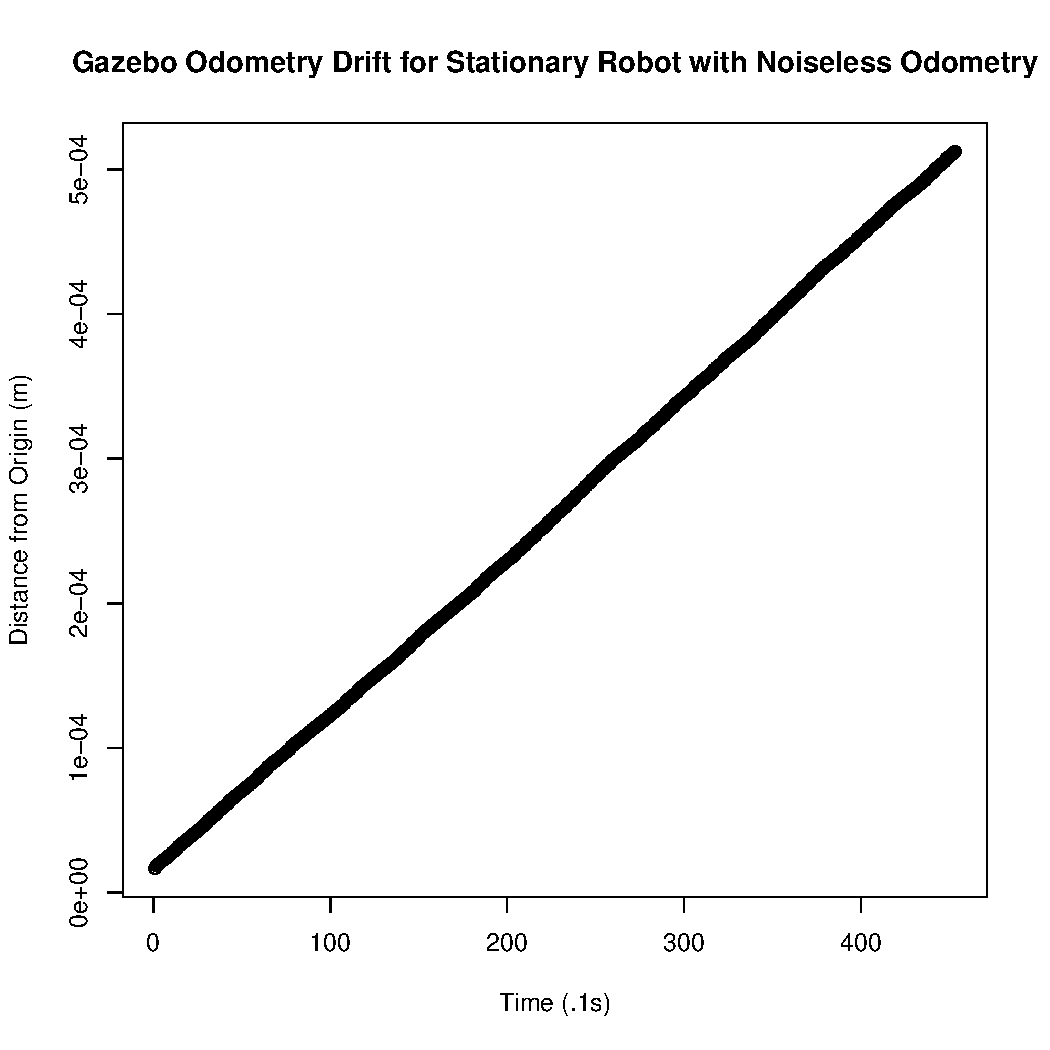
\includegraphics[width=\textwidth, keepaspectratio]{gazebo_odom_drift}
\caption{Gazebo Odometry Drift for a Stationary Robot Over Time}
\label{fig:gazebo_odom_drfit}
\end{figure}

%\subsubsection{IMU}
%TODO maybe reinclude this IMU section, if can solve IMU errors
\subsubsection{Camera}
In the TurtleBot platform, the Kinect camera is used to emulate a Lidar. The depthimage\_to\_laserscan node receives the depth image from the camera, samples a user-defined number of points horizontally along the center line of the image, and uses these distances to create a message as if those distances were determined via a Lidar scan. It is possible to take that Lidar message and add random noise to it via an intermediary node before it is received by the robot node or move\_base nodes. However, Gazebo offers the option of simulating output amplifier noise, which adds Gaussian noise to each pixel in the camera image. This is a much better approximation of our real-world noise, so it is what we used. Based on the recommendations found in the Gazebo sensor noise tutorial~\cite{GazeboSensorNoise}, we used a mean of 0 and standard deviation of 0.007 for our camera's error parameters.

\subsubsection{Pose Estimate}
There are three sources of error in the calculated pose estimate for a detected robot. The first two sources of error are the Lidar error and the odometry error. Calculating the pose involves using the Lidar reading and the robot's current pose to calculate the location of the other robot. Since there is noise in both the odometry and the Lidar, there is noise in this calculation.

The second source of noise is in the projection from the TurtleBot boundary to the center. When calculating the pose of the TurtleBot, our Lidar measurement is not registering the center of the TurtleBot. Instead, it is hitting some exterior part of the TurtleBot. We do not know the relative angle of the two TurtleBots though, nor the angle of contact between the scan and the TurtleBot exterior, so calculating exactly which exterior part of the TurtleBot is being detected is impossible. We know then that the detected point will be no more than 0.2 meters (TurtleBot radius) from the center of the TurtleBot, and testing shows that this error is often between .05 and .1 meters.
%TODO could actually test this and go back to a projection if it's a constant number 

\subsubsection{GPS}
The \gls{faa} produced a report in 2014 about the accuracy of \gls{gps} systems~\cite{FAAGPS}. The data was collected from April 1st through June 30th, 2014 at 28 different locations. The results showed that the \gls{gps} system horizontal measurement error fits a 95\% confidence interval of 3.351m. A mean error was not stated, therefore 0 is assumed. This assumption is possibly inaccurate, though we do not feel it would impact the results of this analysis. Further assuming our data are normally distributed, we model our noise with a mean of 0 and a standard deviation of 1.71 to fit this 95\% confidence interval.

To create the noisy \gls{gps} signal, we take the Gazebo published ground truth odometry, which is delivered in the robot's odom frame, and add it to the robot's initial starting position, which is given in the map frame. This gives us the robot's accurate position in the map frame. Then we sample from our distribution to choose a horizontal error. Once that is selected, we sample from a uniform distribution of $[0, 2\pi)$, and calculate a new location offset from the original location in polar coordinates by the angle and distance selected. This algorithm is shown in \cref{tab:noisy_gps}

\begin{table}[htbp]
\centering
\begin{align}
&x = x_{initial} + \bar{x}\\
&y = y_{initial} + \bar{y}\\
\notag \\
&horiz_{error} = \textbf{sample}(1.71)\\
&\theta = \textbf{$sample_{uniform}$}(0, 2\pi)\\
\notag \\
&x' = x + horiz_{error} \times \cos(\theta)\\
&y' = y + horiz_{error} \times \sin(\theta)
\end{align}
\caption{Algorithm for generating noisy\_gps positions. These are received by the robot at a rate of \SI{0.1}{\hertz}}
\label{tab:noisy_gps}
\end{table}

\end{document}